\documentclass[10pt]{standalone}
\usepackage{tikz}

% TikZ libraries `calc` needed now to tweak bracket.
\usetikzlibrary{backgrounds,fit,decorations.pathreplacing,calc,shapes,arrows}
% Dirac Kets
\begin{document}
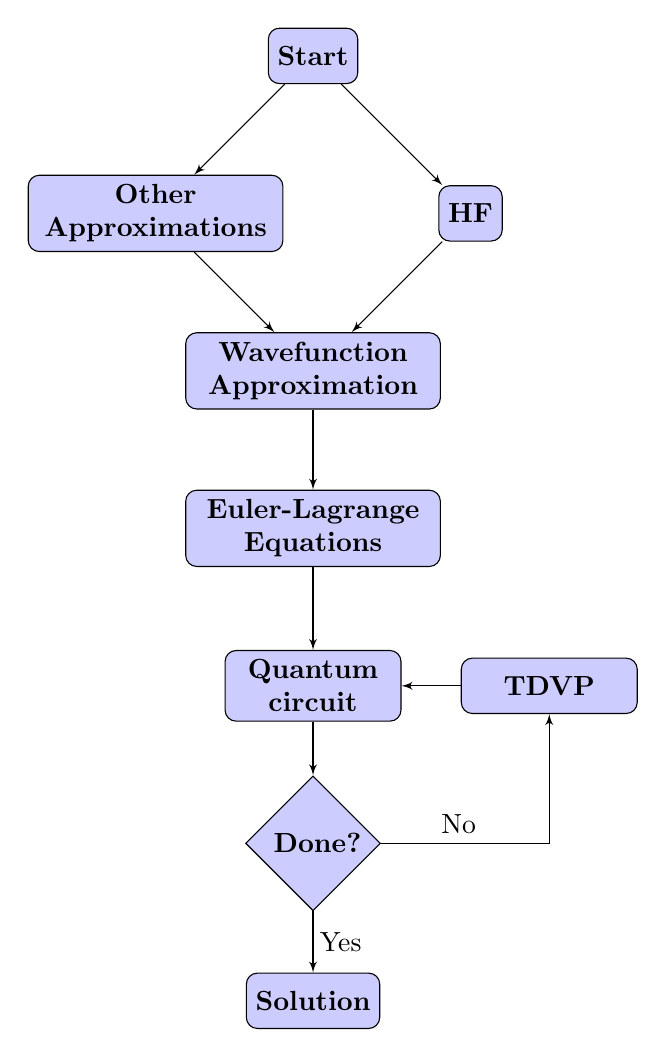
\begin{tikzpicture}
	\tikzstyle{terminator} = [rectangle, draw, text centered, rounded corners, minimum height=2em]
	\tikzstyle{process} = [rectangle, draw, text centered, minimum height=2em]
	\tikzstyle{decision} = [diamond, draw, text centered, minimum height=2em]
	\tikzstyle{data}=[trapezium, draw, text centered, trapezium left angle=60, trapezium right angle=120, minimum height=2em]
	\tikzstyle{connector} = [draw, -latex']
\node [terminator, fill=blue!20] at (0,0) (start) {\textbf{Start}};
\node [terminator, fill=blue!20] at (2,-2) (hf) {\textbf{HF}};
\node [terminator, fill=blue!20, text width=3cm] at (-2,-2) (approx) {\textbf{Other\\Approximations}};
\node [terminator, fill=blue!20, text width=3cm] at (0,-4) (wf) {\textbf{Wavefunction\\Approximation}};
\node [terminator, fill=blue!20, text width=3cm] at (0,-6) (el) {\textbf{Euler-Lagrange\\Equations}};
\node [terminator, fill=blue!20, text width=2cm] at (0,-8) (qc) {\textbf{Quantum circuit}};
\node [decision, fill=blue!20, text width=1cm] at (0,-10) (dec) {\textbf{Done?}};
\node[draw=none] at (1.85, -9.75) (no) {No};
\node[draw=none] at (0.35, -11.25) (yes) {Yes};
\node [terminator, fill=blue!20, text width=2cm] at (3,-8) (tdvp) {\textbf{TDVP}};
%\node [process, fill=red!20] at (3.5,-5) (error) {Error};
%\node [process, fill=green!20] at (0,-8) (success) {Success};
\node [terminator, fill=blue!20] at (0,-12) (end) {\textbf{Solution}};
\path [connector] (start) -- (hf);
\path [connector] (start) -- (approx);
\path [connector] (hf) -- (wf);
\path [connector] (approx) -- (wf);
\path [connector] (wf) -- (el);
\path [connector] (el) -- (qc);
\path [connector] (qc) -- (dec);
\path [connector] (dec) -| (tdvp);
\path [connector] (tdvp) -- (qc);
\path [connector] (dec) -- (end);
%\path [connector] (start) -- (data);
%\path [connector] (data) -- (decision);
%\path [connector] (decision) -- (error);
%\path [connector] (decision) -- (success);
%\path [connector] (error) |- (end);
%\path [connector] (success) -- (end);
\end{tikzpicture}
	% `phase' is used for controlled phase gates (dots).
	% `surround' is used for the background box.
	%\tikzstyle{operator} = [draw,fill=white,minimum size=1.5em] 
	%\tikzstyle{phase} = [draw,fill,shape=circle,minimum size=5pt,inner sep=0pt]
	%\tikzstyle{surround} = [fill=green!30,thick,draw=black,rounded corners=2mm]
	%\tikzstyle{blank} = [fill=green!30]
	%
	%\matrix[row sep=0.4cm, column sep=0.6cm] (circuit) {
	% First row.
\end{document}
